\section{Performance Analysis}
\label{sec:perf}

After we were done with the implementation of MS5, we wanted to test our system to 1) analyze the response times of normal read and write operations, and 2) check the impact of the chatting functionality on the response times. 

320 key-value pairs are used as input for the tests, which were derived from the Enron email set. The way the test works is that clients execute \texttt{PUT}s on all keys, then they try obtaining them back with \texttt{GET}s and in the end all keys are deleted. Each of the three different operations got timed seperatly, so that their efficiency could be compared. The cache replacement strategy in place was Least Recently Used (LRU), which is the default strategy, and the cache size was set to 16, which represents 5\% of the storage size. Before a new set of commands got started, the list of keys got shuffled, which causes both the degree of cache utilization during read operations and the chance of reconnecting to the responsible server to be more or less based on luck.
In order to avoid skewed results, each test was ran five times and the average was taken.

\begin{figure}
	\begin{subfigure}[b]{\linewidth}
	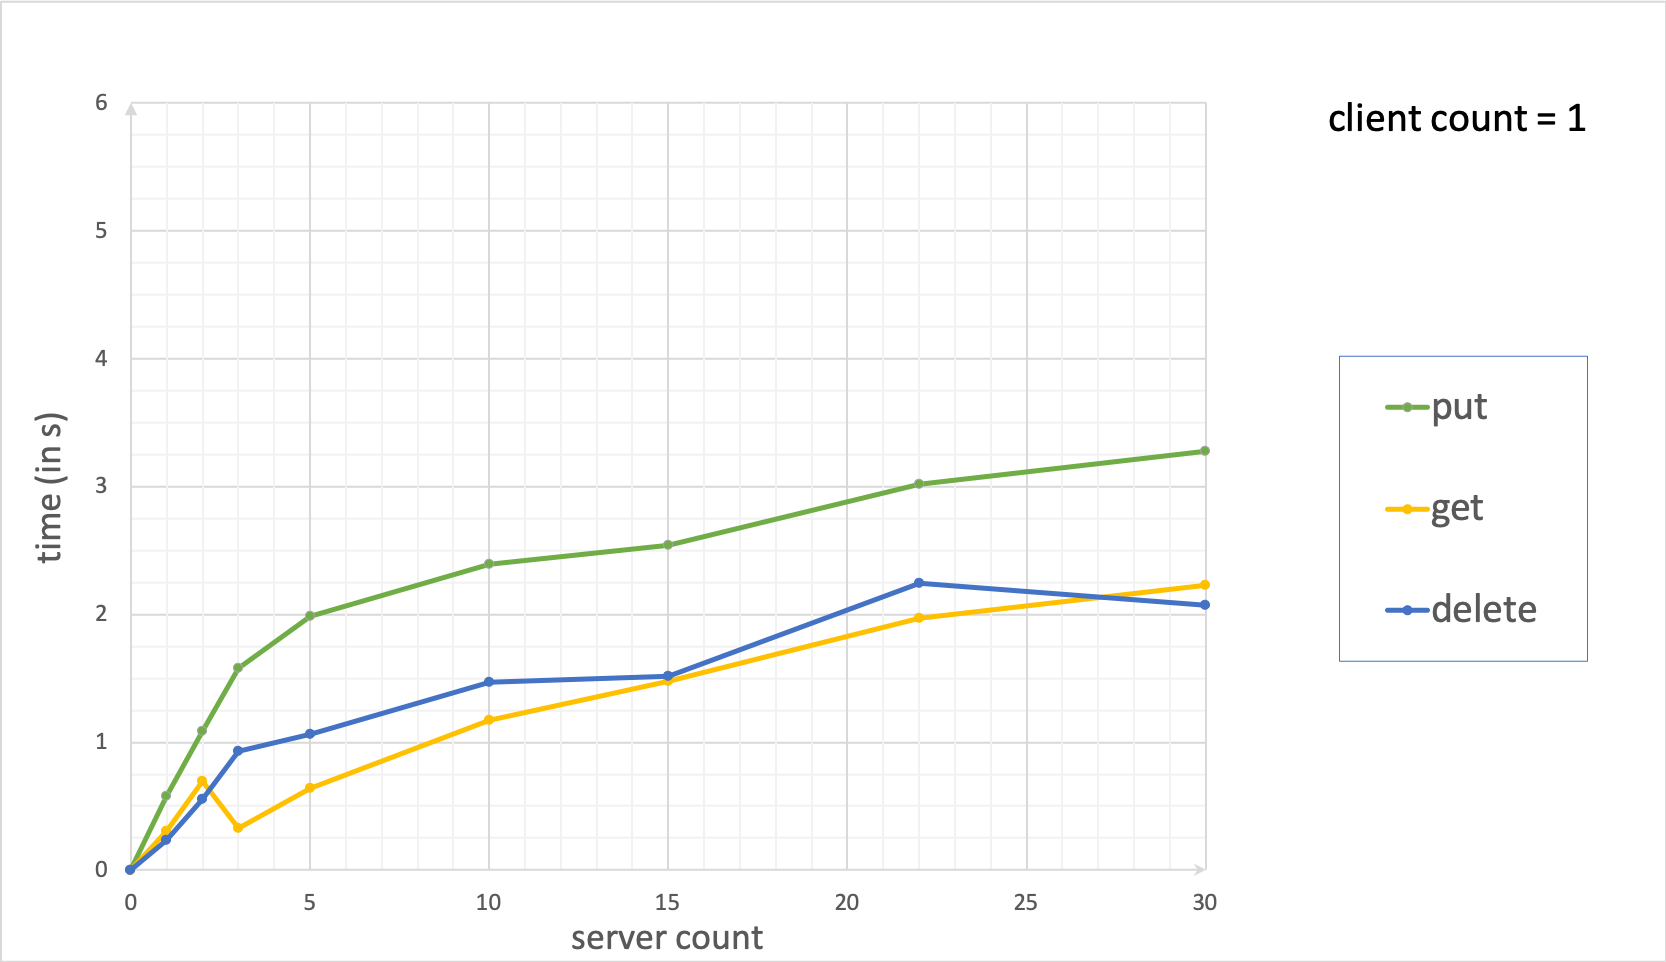
\includegraphics[width=\linewidth]{figures/cc1.png}
\caption{}
\label{fig:perf_cc1}
	\end{subfigure}
	\begin{subfigure}[b]{\linewidth}
	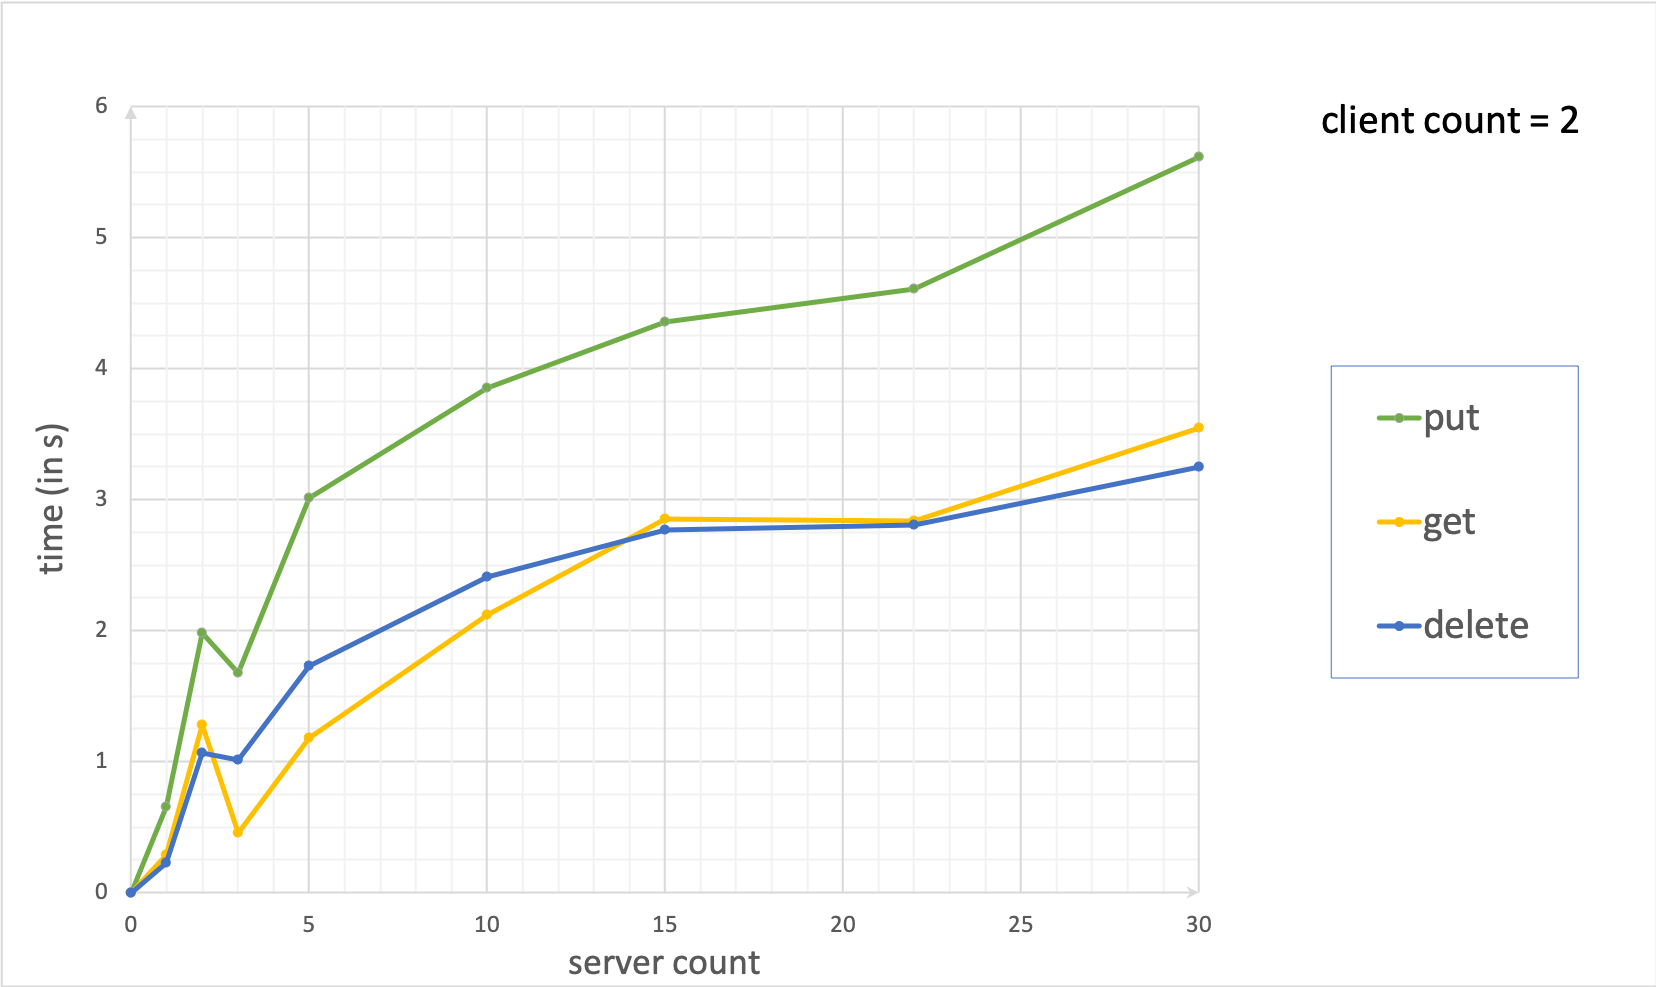
\includegraphics[width=\linewidth]{figures/cc2.png}
\caption{}
\label{fig:perf_cc2}
	\end{subfigure}
\caption{Key-value servers performance}
\label{fig:perf_cc}
\end{figure}

In figure \ref{fig:perf_cc}  we vary the amount of key-value servers and measure the time 320 operations took. At first glance, it is clear that adding an extra client in \ref{fig:perf_cc2} leads to lower response times, since double the amount of requests need to get processed by the servers. Otherwise, in both graphs \texttt{PUT} operations take the most time, because each time the disk has to be accessed and a file has to be written. Even though deletetion manipulates data on disk as well, files just have to be located and removed from the directory, with no need to open them. \texttt{GET}s usually took the least amount of time, since disk access is not always necessary. A significant drop of read response time can be noticed at the three server mark due to replication just getting started. At that point, no reconnection is required for the read commands, owing to the fact that all three servers are now responsible for read operations on all keys. The chance of a reconnection being needed is equal to \begin{math}1-\frac{3}{N}\end{math} with \begin{math}N\end{math} being the amount of key-value servers running. As apparent by the formula, the chance decreases as the server count increases, leading to the rise seen later on in the graphs. 


\begin{figure}[h]
	\centering
	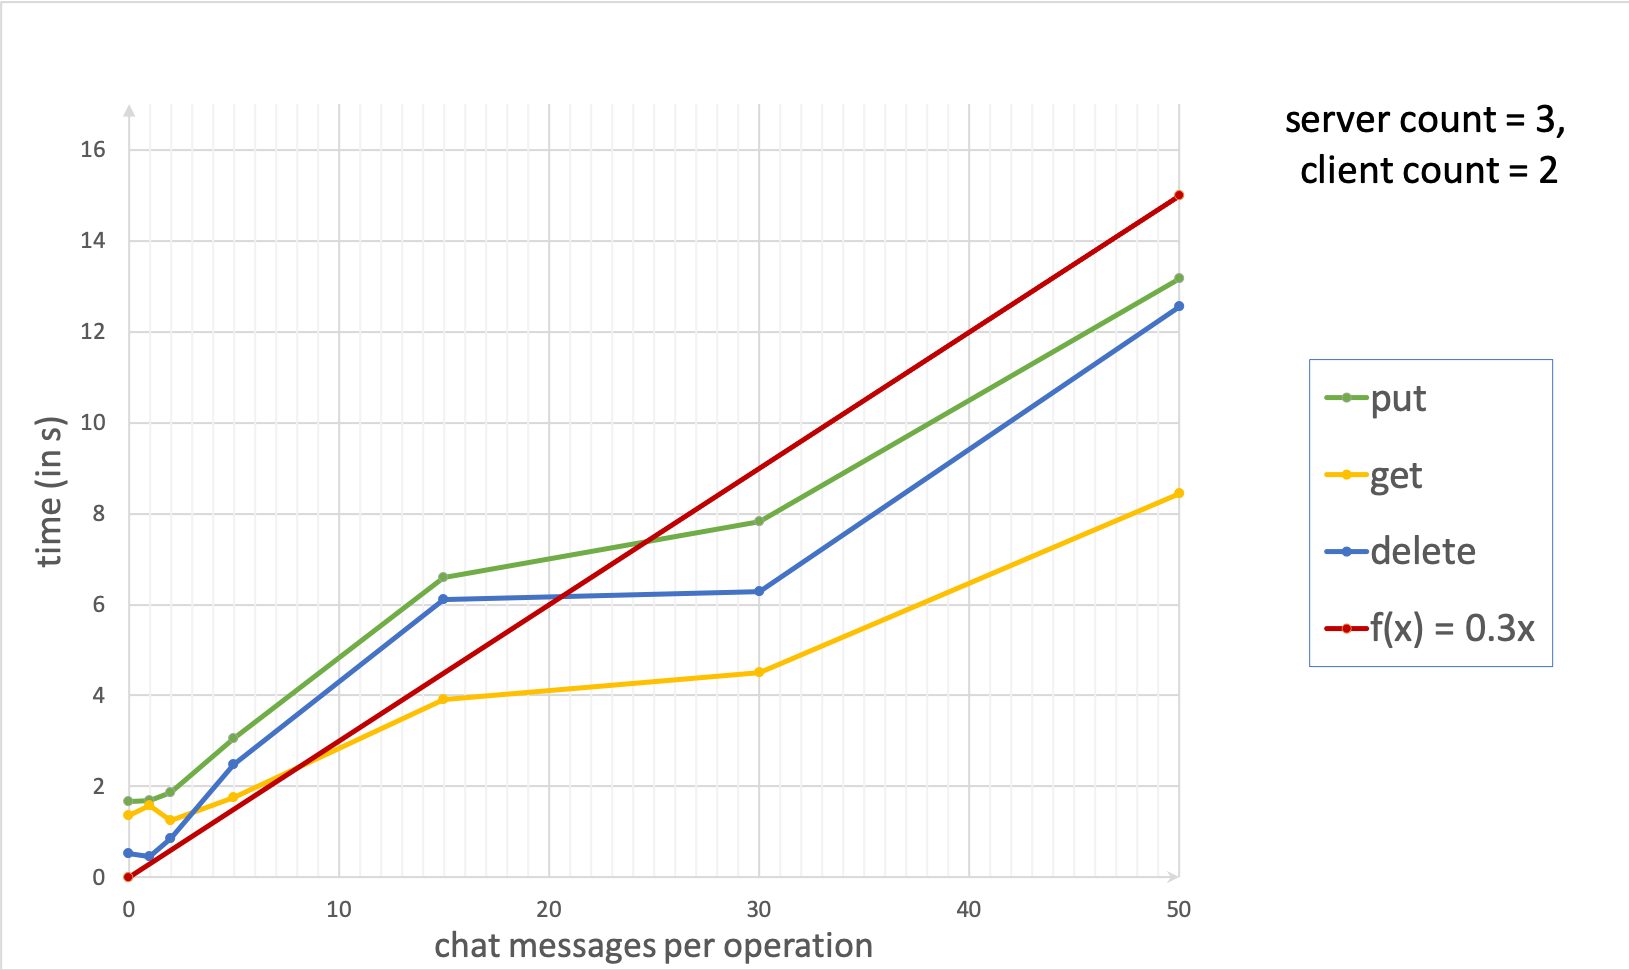
\includegraphics[width=\linewidth]{figures/chat(linear).png}
	\caption{Key-value servers performance in chat mode}
	\label{fig:perf_chat_lin}
\end{figure}

After we have evaluated the response time for the normal database operations, we try executing these same commands but inside a chatroom. For our testing purposes, we had two clients in the same chatroom perform those commands. The difference here is that, unlike in figure \ref{fig:perf_cc2}, where each client directly contacts the key-value servers, only one common bot is utilized by both users. After each command, the user would send a certain number of chat messages as depicted on the X-axis, in order to simulate a general use case scenario of our system. Graph \ref{fig:perf_chat_lin} depicts the increase in response time in relation to the chat messages sent.
When few messages are sent, the extra time required compared to the normal database operations seems unnecessary. 
However, the response times do not grow at the same ratio as the chat activity, but rather roughly follow the path of the function \begin{math}0.3x\end{math}. That means that for each additional chat message per operation per client (equal to overall \begin{math}320 * 2 = 640\end{math} extra messages), the system is slower by just about 300 milliseconds. In one extra second, more than 2100 messages can get exchanged.